%=============================================================================
% DESIGN

\documentclass[../mpaper.tex]{subfiles}
\begin{document}

As we have discussed the importance of User Experience and Human-Centered Design, we educate our implementation by outlining three fictional personas for our design.

\begin{itemize}
    \item Developer 1: David is a 35-year-old senior software developer who graduated with a Bachelor's degree in Computing Science from the University of Edinburgh. He has been working in the industry for over 10 years, with experience in large organizations such as RBS, Skyscanner, and Amazon. He is now the tech lead for a SaaS startup based in Edinburgh. David is a perfectionist who values efficiency, scalability, and maintainability in software development. He has experience working with various programming languages such as Java, Python, and JavaScript and is comfortable working with both front-end and back-end technologies.

    \item Developer 2: Sarah is a 27-year-old junior software developer who graduated with a Master's degree in Graphic Design from the Glasgow School of Art. After graduation, she taught herself programming over the last two years by following Python tutorials \& exercises on YouTube. Being a creative and visual thinker, Sarah enjoys designing user interfaces and user experiences (UI/UX), but she is new to the world of software development eager to learn more about programming languages and web development frameworks.

    \item Developer 3: Alex is a 28-year-old software developer who graduated from a programming boot camp three years ago. They enjoy solving complex problems with a keen interest in software development. They are proficient in developing features and documenting those features, making them an essential member of a SaaS startup team. Alex has experience working with React and Node.js and is eager to learn new technologies and frameworks to improve their skills further.
\end{itemize}

The three developers, having different backgrounds and skillsets, are working in the same SaaS startup as a team working to provide a website for the startup that displays their services, handles transactions and allows employees to write blog posts with SEO\footnote{Search Engine Optimisation}. They must choose the right tools that will facilitate the entire development and ask questions like "\textit{how fast will it enable us to create the MVP\footnote{Minimal Viable Product}?}", "\textit{does the tool have documentation and integrate well into an ecosystem while keeping dependencies low?}" and "\textit{will it ensure that the codebase is maintainable for the future (of the company)?}" - a lot of decisions tie to the experience developers would have working with the tool. % For this \sout{scenario} example, say they choose to use Next.js (based on React) and other dependencies like styling libraries (TailwindCSS), eCommerce integrations (Stripe), authentication handlers (Supabase) and content management systems (Sanity) -- all chosen wisely as they are backed by well-funded organisations and ensure development of enterprise-level applications; if any core dependency had an uncertain future, the functionalities of the website could collapse. They must integrate into each other, referring to documentation for each dependency - unoptimised integrations could increase technical debt.
They must also ensure that despite different skills and subjective DX, the development of the code itself is \textit{objective}, i.e. it does not depend on who is writing the code and everything is consistent, so some rules must be chosen such as code style, directory structure, pipeline tests, automated hooks, and other similar factors. Code reviews also improve consistency but they are known to be big blockers in productivity and time-consuming \cite{canedoFactorsAffectingSoftware2019} costing the company time and money.

A big part of the funding is used to compensate the developers (their pay), so they require detailed timesheets so that the data can be used to educate estimates and shared with investors for appropriate budgeting. The company could also use monitoring software, but this would be problematic -- the software may not be specialised in studying developer activity requiring manual review and it could make employees conscious of their activity. The code repository shows activity, however, it only contains objective metrics and discrete events, such as commits, timestamps, issues closed, and SLOC, not covering the real effort of the developers when they're not writing code (reading documentation, doing code reviews, etc). Instead, the team can be provided with a hybrid monitoring tool that enables them to review their activity themselves, breaking down their efforts (see \autoref{fig:example_timeline}), and use it during retrospective meetings.

\begin{figure}
    \centering
    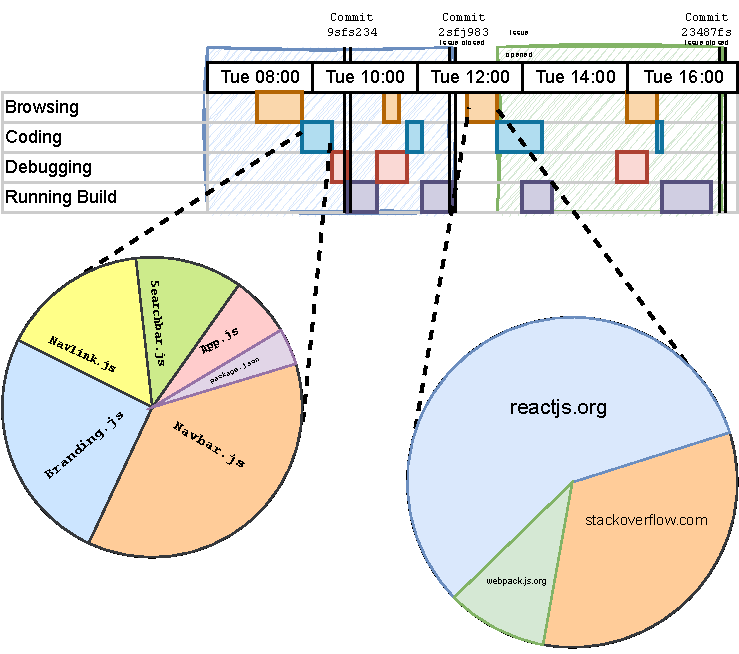
\includegraphics[width=0.45\textwidth]{sampleviz.pdf}
    \caption{Example of efforts spent on a timeline}
    \label{fig:example_timeline}
\end{figure}

Think of a scenario where the team were reported a bug on a page of their pilot prototype website with error-message "\texttt{TypeError: cannot read property of undefined (reading 'toString')}". This prototype uses a standard React front-end with a Django REST Framework back-end. To investigate this bug, there are lots of questions to be raised.

\begin{itemize}
    \itemsep-2pt
    \item "\textit{why was this not covered in tests?}"
    \item "\textit{what does the documentation say? what does Google say? what are the search keywords? will it trim down results and give an exact response?}"
    \item "\textit{why does it happen only one page? is it the routing library or the page component code?}"
    \item "\textit{is the code written in JavaScript or TypeScript? if TypeScript, the compiler should locate the issue}"
    \item "\textit{what does the traceback say? is the React app being served as a static asset through Django with Webpack building the compiled \texttt{main.js} in watch mode?\\if so, traceback is useless}"
    \item "\textit{if it is being served through Django, the file may also be cached in the browser and not reflect latest changes, so does cache need to be cleared every time (frustrating) or it needs to be tested on incognito?}"
\end{itemize}

The fix, carried out by Sarah over tasks outlined in \autoref{fig:issue-flow}, just involved adding a condition to an \texttt{if} statement with commit diff as \texttt{+1 addition -0 deletions}. This may be a minor change, but the dashboard would verify Sarah's actual efforts that went into making this change creating a good point of conversation for the team in their retrospective so that they can plan a refactor and improve debugging for their project to provide better DX with faster fixes. % A high-level overview of sample tasks in the workflow can be seen in \autoref{fig:issue-flow}.

\begin{figure*}
    \centering
% - Planning (create/pick up backlog) - do estimates if not assigned (main area)
% - Study issue, look at description and story. Understand code changes - is it bug? then replicate it. is it feature? understand how it works and write tests first if u want
% - Create issue branch
% - Start to code on branch, local development
% - Look at documentation, go back
% - Write tests, run tests
% - Commit, push branch, pipeline, CI
% - Create PR, link issue, describe PR, do code-review
% - Merge \& release
% - Retrospective
    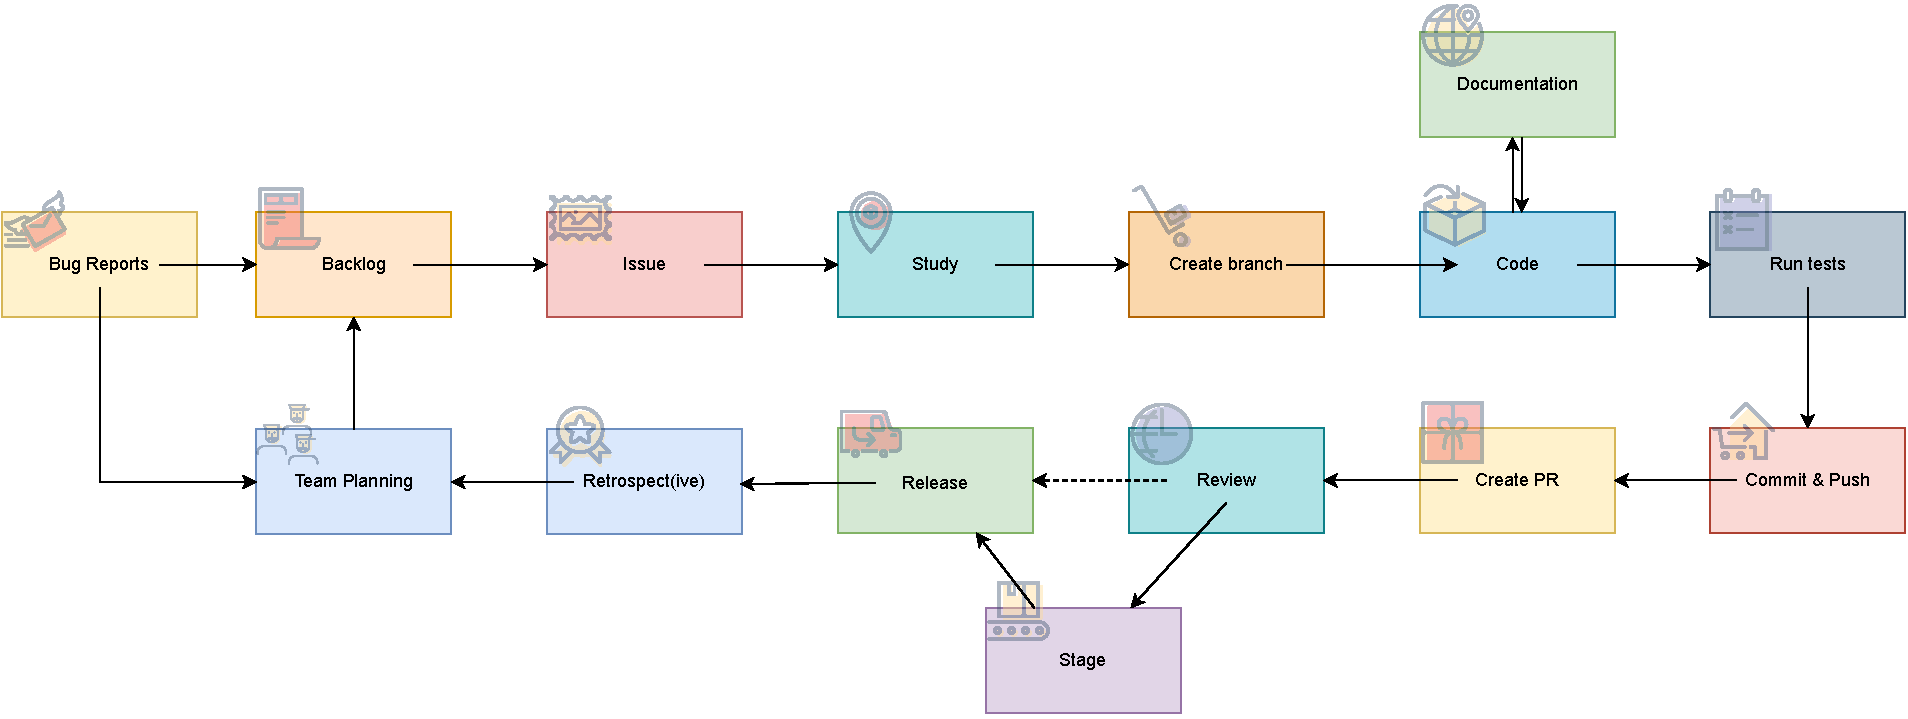
\includegraphics[width=0.95\textwidth]{issue-flow.pdf}
    \caption{Workflow of a developer with an issue}
    \label{fig:issue-flow}
\end{figure*}

% \subsubsection*{Experiment Design}

% In addition to user-driven development with the scenario created in this section, our experiments were also partially planned ahead of implementation so that the designs could be adjusted \& improved iteratively ensuring that the developed solution would be evaluated successfully. This included carrying out a longitudinal study with developers working on projects with their teams on a deadline in an agile discipline. They would follow the cycle of sprint planning \& retrospectives and the tool should improve their meetings and task estimates. More discussed in \autoref{sec:Evaluation}.

\subsubsection*{Application Design}

Remote repository hosting services (such as GitHub, GitLab and Bitbucket) provide their unique set of features to enable developers to be able to progress on their development processes in a disciplined, streamlined manner if they prefer; this includes issue tracking, forking, wiki documentation, etc. While wiki documentation is designed as a separate repository with the same name as the main source code repository but with a \texttt{.wiki} suffix, many projects also tend to keep consistent documentation in a \texttt{docs/} directory that gets compiled and deployed to different sources. The repository README, however, has been a critical part to development; this acts as the home landing page to the project and developers tend to spend time in writing and/or understanding it. With the power of Markdown, it has become easy to write and preview the document. Moreover, Markdown Badges (or Shields) are a popular way to display information about the project such as license, code-size, pipeline status, out-of-date dependencies, etc \cite{trockmanAddingSparkleSocial2018} - this has made the README as a good source of all information required on the "landing page". This idea is the inspiration. Markdown is limited to the simple syntax; other services exist but they also have limitations such as being outside the SCM, limited metric options and unpredictable payment plans.

The proposed solution developed a dashboard that is integrated into the developers' workflow, through their Text Editor or IDE\optionalnote{Integrated Development Environment}, and displays their efforts spent on completing tasks on their repository to ensure that they are aware of their precise development activity. The system uses a highly-integrated \& modular architecture to enable quick and adaptive customisation of the dashboard if developers are only interested in certain metrics -- similar to fitness applications like Google Fit and Fitbit that allow toggling of graphs and integration with third-party services, essentially making our tool to be a fitness app for software projects.

\subsubsection*{Visualisations}

For the initial version of the dashboard, we needed to study and provide default visualisations that could interest developers and show potential for more metrics. We planned to display their sprint as a timeline. The information that developers mostly look for in their repositories are commits, issues, and pull/merge requests. We can use the time difference between two commits (to look into what they were working on), issue opening \& closing (to look into how they were working), and pull request being created \& merged/closed (to look into how they were reviewing) as a continuous event and display activity between those timestamps.

The visualisations must be unique from the ones that hosting services provide; they usually provide a contribution graph but they only consider commits while creating issues and pull requests is an equally important task. Teams may also want to see how their week was spent if sprints last over multiple weeks. Sunburst charts of their time would also provide useful, comprehensive breakdowns of their time. For example, say Alex spent 4 hours on closing an issue. 60\% of the time was spent coding and within that 60\%, 40\% was spent on \texttt{AboutPage.js}. Finally, David may want to routinely review the repository file-by-file to see when the last changes to each file were made. If a file is changed frequently, that may not be optimised and would need to be broken down, or if a file is not changed frequently (say \texttt{package.json} or \texttt{requirements.txt}), it may be outdated. In this case, a form of a file-heatmap would be very useful.

\end{document}
